\documentclass[12pt]{report}
\usepackage{graphicx}

\begin{document}
The main folder is "SYS-101". In that folder, we have "build.sh" as the script file. The script file runs and gets the output of "main.c", "diagraph.dot", and "plot.R". It then combines the output of the files into "createPdf.pdf" using "createPdf.tex". After this is done, all the generated files are cleaned up.

\begin{figure}[h]
\centering
\caption{Block Diagram}
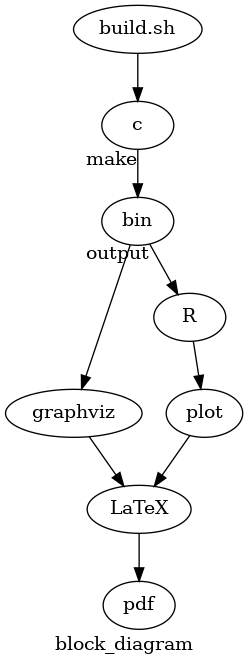
\includegraphics[height = 0.7\textheight]{image.png}
\end{figure}

\begin{figure}[h]
\centering
\caption{Plot}
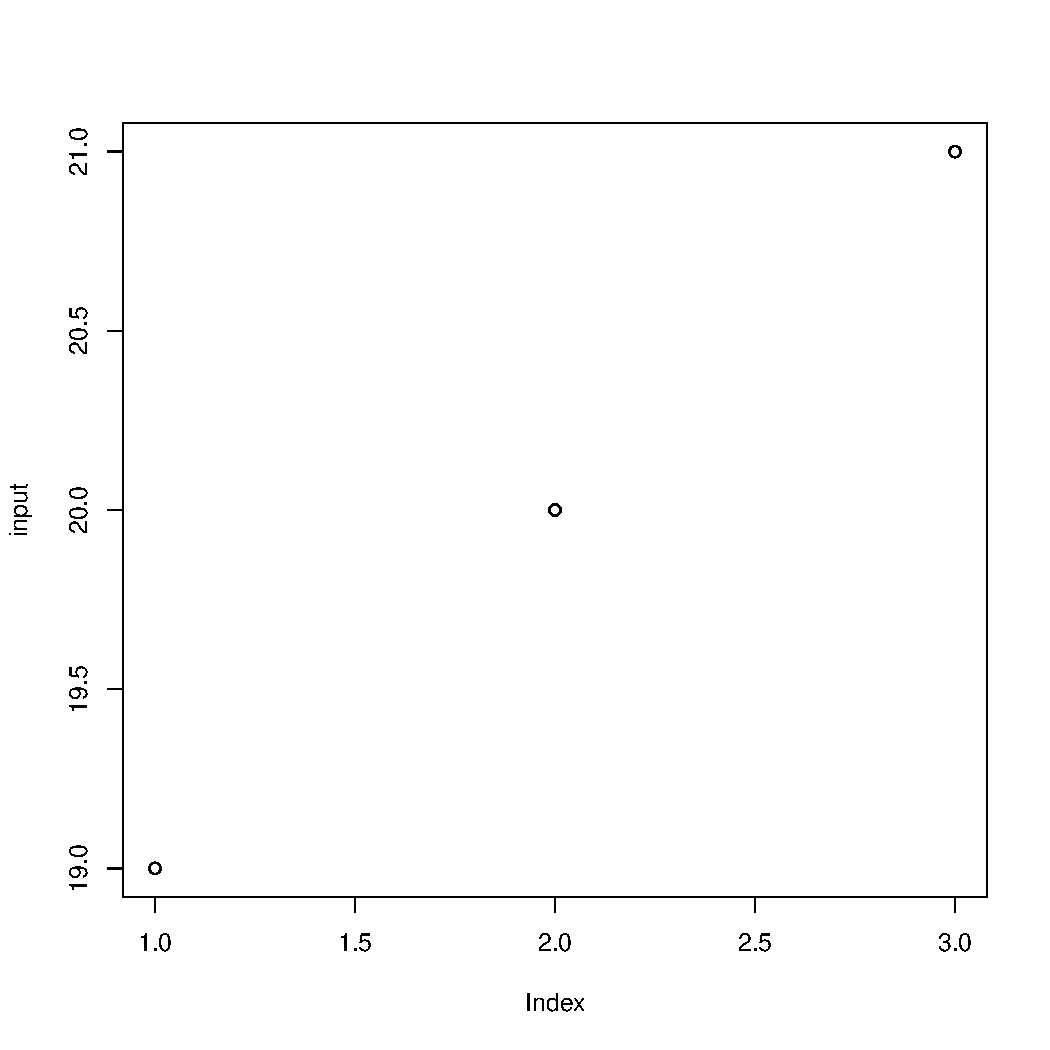
\includegraphics[height = 0.8\textheight]{Rplots.pdf}
\end{figure}

\end{document}